% 2400 signs per page setup:
\documentclass[a4paper, 12pt]{article}

\usepackage{geometry}
\usepackage{amsmath}
\usepackage{color}
\usepackage{graphicx}
\usepackage{array}

% images alongside text
\usepackage{wrapfig} 
\usepackage{hyperref}
\usepackage[parfill]{parskip}

% blank pages
\usepackage{afterpage} 

% #http://ctan.org/pkg/{fancyhdr,graphicx,lastpage}
\usepackage{fancyhdr,graphicx,lastpage}

% get the degree symbol
\usepackage{gensymb} 

% subfigures inside of normal figures
\usepackage{subcaption} 

% Glossary / Abbrevations list
\usepackage{glossaries}

% Include other files into document
\usepackage{subfiles}

% Bibliography and refrence manager with Biber
\usepackage[backend=biber, % compile with biber (pdflatex %; biber %; pdflatex %; pdflatex %)
            sorting=none %  none means sort by appearance
            ]{biblatex}
\addbibresource{./sources.bib} % take bibliography resources from this file

% Define margins for page setup
\newgeometry{vmargin={30mm}, hmargin={30mm}, tmargin={30mm}, bmargin={30mm}}

% Shortcut path for graphics
\graphicspath{ {./src/} }

% Header/Footer setup:
\fancypagestyle{plain}{
  \fancyhf{}                                       
  \fancyhead[L]{Surface-EMG Processing \& Classification for Muscle Interfaces}
  \fancyhead[R]{}
  \fancyfoot[L]{Thomas Alexgaard Jensen (tjens18) \\ University of Southeren Denmark}
  \fancyfoot[R]{\thepage\  / \pageref{LastPage}}
}

% Set page style to plain.
\pagestyle{plain} 

% Define Title Page information
\title{Surface-EMG Processing \& Classification for Muscle Interfaces}
\author{
\\University of Southeren Denmark
\\
\\Supervisors: 
\\Poramate Manoonpong (poma@mmmi.sdu.dk)
\\Xiaofeng Xiong (xizi@mmmi.sdu.dk)
}
\date{Date: }

% norm symbols for math
\newcommand{\norm}[1]{\lvert #1 \rvert}

% Explanation setup, used for specific words explanation
\newcommand{\explanation}[2]{
\textit{#1: }{#2.}
}

\begin{document}

%1.highlighting what you have achieved
%2.the plan for the rest months 

\section{An Overview of the Acheivements and Holdups}
\subsection{The Plan According to the Contract}

I have taken the original development plan from the contract to visualize my progress.
In the diagram, \textbf{red squares} are completed tasks, and \textbf{red circles} are the tasks i am working on, but have experienced lab difficulties.

\begin{center}
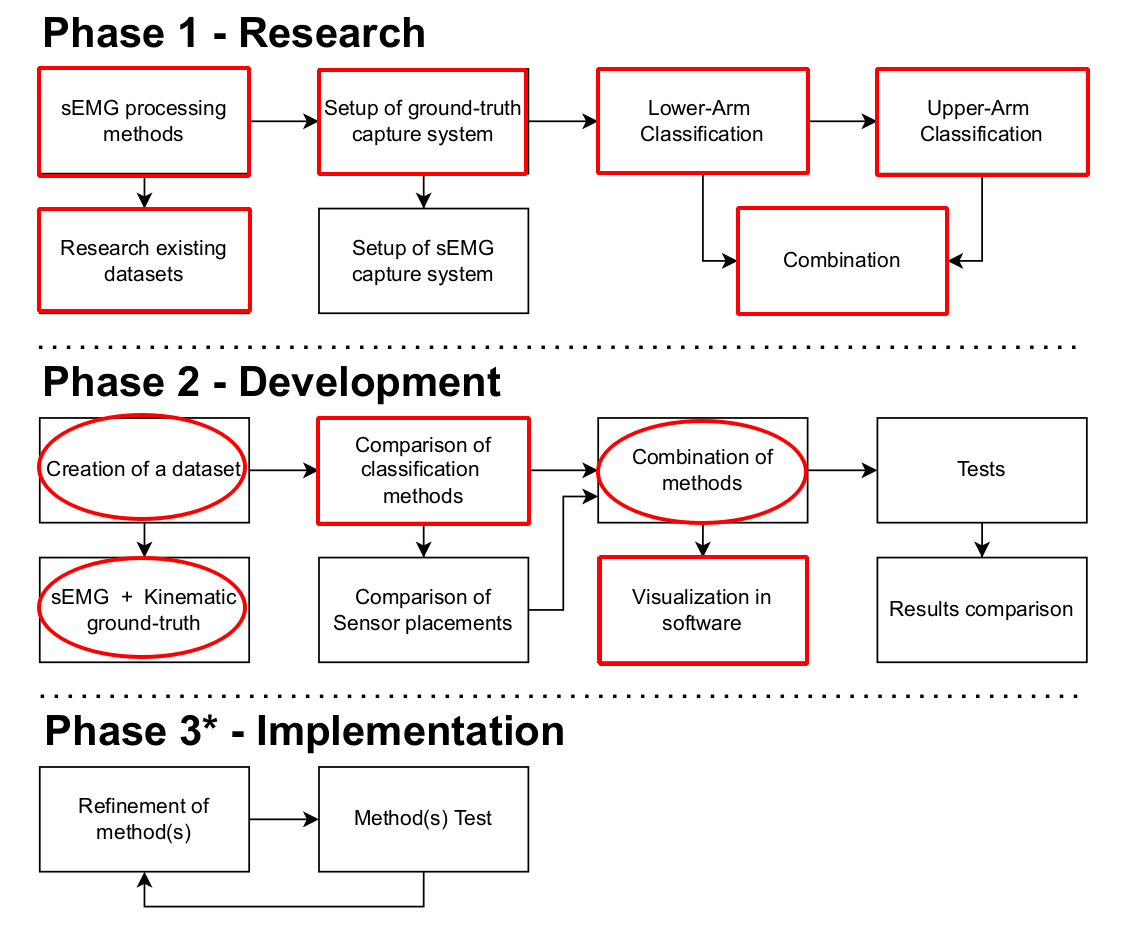
\includegraphics[width=0.99\textwidth]{meta-graph-progress.png}
\end{center}

\subsection{Pitfalls and Holdups along the development}

I have spent a lot of time on software that ended up not being comtatible or working in the way it should be expected to, noteably:

\begin{itemize}
\item Finding and using an existing prosthetics simulation proved difficult, with software not working, being paid/unavailable, deprecated etc. 
\item Setting up Gazebo and developing a working simulation took too much time, so i changed to CoppeliaSim.
\item The Camera system having a hard time giving poses for the 3D markers.
\item Connection issues with hardware synchonization
\end{itemize}

\subsection{Current Acheivements}

The things i have accomplished so far in the development period:

\begin{itemize}
\item Created a rigidbody, Simulated hand in CoppeliaSim, that is anatomically correct, ROS communication compatible and able to be controlled into different life-like poses.  
\item Designed different types of Neural Networks able to perform regression of joint angles based on sEMG inputs from the muscles of the lower-arm.
\item Created a motion capture glove that is able to be used in lab to get joint angles of the hand while recording muscle activity.
\item Read, Summarized \& Sorted state-of-the-art techniques of prosthetics control for the report. 
\item Defined a recording session test based on state-of-the-art methodology.
%\item Written half of the required report
\end{itemize}

\subsection{Plan for the Rest of the Thesis}

I plan to focus on the things that are most important for my thesis, the things listed below are what i find important, but i hope you would share your perspective on what my focus should be:

\begin{itemize}
\item Get hardware synchronization to work and create a dataset using the recording glove and the sEMG sensors for the lower-arm.
\item Once the above works, Explore fine tuning of my created networks for the dataset.
\item Create tests where i also place sensors on the upper-arm/ shoulders.
\item Test the hypothesis that we can use the upper-arm/shoulder data to further increase regression.
\item Test and assess the results of the AI-based regression in the prosthetic simulation.
% \item create a kind of sleeve with recordning markers on it so that i can 
\end{itemize}

I hope to have multiple people contribute to the dataset as we originally planned, but i think it will depend on when i get the system properly working.


\end{document}
